\documentclass{eplmastersthesis}
%TODO: fixing the scale: the more points, the more everything goes to the origin?
%\usepackage[a4paper,width=150mm,top=25mm,bottom=25mm,bindingoffset=6mm]{geometry}
%\usepackage{graphicx}
%\usepackage{fancyhdr}
%\pagestyle{fancy}
\usepackage[backend=biber]{biblatex}
%\usepackage[acronym,nomain,nonumberlist]{glossaries}
\usepackage{float}
\usepackage{textcomp,gensymb}
\usepackage{csquotes}
\usepackage{booktabs}
\usepackage{siunitx}
\usepackage{hyperref}
\usepackage{multirow}
\usepackage{caption}
\usepackage{subcaption}
\usepackage{amsmath}

\usepackage{mathtools}
\usepackage{amssymb}
\usepackage{tabulary}

\usepackage{pgfplotstable} % Generates table from .csv


\pgfplotsset{compat=1.9}
\hypersetup{
    colorlinks,
    citecolor=black,
    filecolor=black,
    linkcolor=black,
    urlcolor=black
}

\setlength{\heavyrulewidth}{1.5pt}
\setlength{\abovetopsep}{4pt}

\addbibresource{references.bib}

\graphicspath{ {images/} }

\title{Drone Navigation in Confined Spaces}
%\subtitle{Subtitle (optional)}			% Optional subtitle
\author{Boris \textsc{Dehem}}
\speciality{Mathematical Engineering}
%\options{Option(s)}		% If required by program commission mention options
\supervisor{Julien \textsc{Hendrickx}}
\cosupervisor{François \textsc{Wielant}}	% 2nd supervisor name if applicable
\readertwo{Christophe \textsc{De Vleeschouwer}}
%\readerone{François \textsc{Wielant}}
\years{2016-2017}


% Generate the glossary
\begin{document}
%Term definitions
%\newacronym{uav}{UAV}{Unmanned Aerial Vehicle}
%%\newglossaryentry{caca}{name=ABC, description={Allo Boris Caca}}

%\maketitle					% To create front cover page
%\thispagestyle{empty}		% To suppress header and footer on the back of the cover page
\pagenumbering{roman}

%\chapter*{Abstract} Abstract goes here

%\chapter*{Dedication} To mum and dad

%\chapter*{Declaration} I declare that..

%\chapter*{Acknowledgements} I want to thank...

\tableofcontents

\newpage
\pagenumbering{arabic}
\chapter{Introduction} %11
%%Introduction (chpt1)
\section{A brief history of drones}
\Glspl{uav} (Unmanned Aerial Vehicles), more commonly called drones, are defined as flying vehicles without human operators on board. They can be remote-controlled, or controlled by on-board computers. The earliest recorded use of \glspl{uav} dates back to 1849, when Austria launched about 200 unmanned balloons armed with bombs against de city of Venice \cite{anthology}. Due to unfavorable wind conditions, this attack failed, and the experiment was not repeated. The first functional UAVs were made towards de end of World War 1 and their use was, like the Austrian balloons, military. One example is the Kettering Bug (Figure \ref{fig:ketteringbug}), which was a torpedo with wings and a propeller developped by the US Army in 1918 \cite{dronesww1}.
\begin{figure}[H]
  \centering
  \includegraphics[width=0.5\textwidth]{kettering_bug.jpg}
    \caption{The Kettering Bug (1918)}
    \label{fig:ketteringbug}
\end{figure}

Throughout the 20th century, UAVs become more and more sophisticated, and were used more and more, but always for military purposes. In the more recent years, civilian UAVs have started to appear on the markets and their number quickly exceeded that of military UAVs. In february 2017, the FAA (Federal Aviation Administration) of the United States estimated that around 1.1 million units were in use in the US alone, and expected that number to rise to 3.55 million by 2021 \cite{consumerdronesbythenumbers}. These civilian drones are very different from military drones, in both their form and their function: civilian drones are usually smaller, and use rotors to take off vertically. They are used in a wide variety of applications.

\section{Motivation}
The ability to remote-control small and agile flying objects over large distances through the air, and to bring them to previously inaccessible locations, makes many new things possible. With the increasingly lower prices and better performances of civilian UAVs, people keep finding more and more uses for these high-tech gadgets. Some examples of these applications are: crop monitoring in agriculture \cite{agriculturaldrones}, delivery of mail or parcels, construction \cite{batiravecdesdrones}, cinematography, entertainment, or search and rescue operations. In all these applications, the more autonomous a drone is, the more efficient it will be at its task. One of the main challenges to achieve autonomy is for an UAV to be able to correctly identify its surroundings, and localize itself within them. In outdoor environments, GPS systems allow UAVs to know their position with great accuracy, but this is not possible in GPS-denied environments, such as indoors. The main subject of this thesis will be fully autonomous navigation by a quadcopter in a GPS-denied environment.

\subsection{Ethical considerations}
The new possibilities brought by drones also pose ethical questions about security and privacy. Even though this technology can improve people's quality of life, it also has the potential to diminish it. If drones start to be widely used comercially, we could reach a point where the sound nuisances that they cause seriously impacts people who live in densely populated areas. Also, they can make us feel less at home, knowing that we could be observed from the sky. For this reason, it is important to adopt strict reulations regarding the use of drones in public spaces. Fortunately, many countries are already adopting legislation in this direction.


\section{Context}
This thesis is part of a project at the UCL that spans over several years and several masters theses. This project was launched by professor Julien Hendrickx in the 2012-2013 academic year, and had as long-term goal to develop a program that would enable low-cost UAVs to navigate autonomously in indoor environments. This means creating a map of their environment, localizing themselves in this map, and avoidig obstacles during exploration, using only on-board sensors. Another goal is to allow several drones to collaborate to speed up exploration. Five theses have already been written on this subject, each taking the work of the previous a little further.
\paragraph{2012-2015: First three theses}
In each of the three academic years (2012-2013, 2013-2014, 2014-2015), one masters thesis on the subject of indoor navigation for autonomous low-cost drones was written. These masters theses formed the base of the future work. They implemented visual SLAM methods to allow drones to build a two-dimensional map based on keypoints (first red pucks, then visual landmarks that the drone detected from a textured field of view), and to localize itself within this map. During this time, inter-drone communication was also established, and was used to allow a drone to communicate the location of a target to another drone.

\paragraph{2015-2016: Recent work}
Last year, two groups of students simultaneously wrote theses on this subject. Before doing so, they joined forces to reimplement what had been done previously, but using the ROS interface, an interface to work with robots that would make many things simpler, and allow more flexibility (see section %%TODO for more).
The work of the first group of students allowed a drone to search and follow a mobile target, and call a second drone to continue this task when its battery was low.\\
The second group of students extended to SLAM algorithm to allow to use a 3D map to localize the drone. Unfortunately, they did not implement triangulation to allow to project seen points into 3D space, but rather made the assumption that all points were located on the ground when building the map. The end result was a drone capable of using a 3D map to localize itself, but not capable of building one from its observations.


\section{Objectives}
For my own thesis, my goal is to continue the work of last year's second group, to allow true 3-D SLAM: to build a 3D map based on observations by the monocular camera. To achieve this goal I will follow the following steps:
\begin{itemize}
\item Research the current state of the art for 3D Keyframe based monocular visual SLAM
\item Implement a way to triangulate points based on observations
\item Bundle Adjustment
\item Dense reconstruction
\item Obstacle Avoidance
\end{itemize}

\section{Structure}
%TODO after the rest is done


\chapter{State of the art} %8
%% State of the art (chpt2)
\chapter{State of the art} %8
We begin this work by researching the state of the art in drone hardware, computer vision, and SLAM solutions. All three of these are very active topics with frequent innovations, and we will explore some of them.

\section{Drones}
When talking about autonomous drone navigation, it is important to be aware of what the current hardware is capable of doing, and how we can expect it to evolve in the near future. There is quite a large choice of low-cost drones available to choose from on the market. For civilian UAV's, a tradeoff has to be made between performance (speed, agility, accuracy of sensors, power of embedded computers), battery life, and price. However, it is still a relatively young market, and each year, new drones are created that improve on these quantities.

\subsection{Number of rotors}
Multirotors, or multicopters, are defined as rotorcrafts with three or more rotors. Having more rotors enables them to maneuver in 3D space with fixed-pitch rotors, unlike helicopters, which have articulations at the bases of their rotors. The most common multirotors have 3, 4, 6, or 8 rotors, and are respectively called tricopters, quadcopters (or quadrotors), hexacopters, and octocopters. Having more rotors has the advantage of giving more agility, at the cost of more energy consumption, and therefore a shorter battery life.\\

A free solid object in 3D space, such as a multicopter, has 6 degrees of freedom: 3 for translation and 3 for rotation. To be able to directly control each of these 6 degrees of freedom, it must be possible to give 6 independent controls to the drone. This means that tricopters and quadcopters are always under-actuated: they can't directly control all 6 degrees of freedom.\\

For example, quadrotors whose rotors are all in the same plane (as is almost always the case), can directly control all three of their rotational degrees of freedom, but only one translational degree of freedom, as they can only accelerate in the direction parallel to the rotation of their rotors. Therefore, to control their position in the plane perpendicular to the direction of gravity, they have to first adapt their roll and pitch, so that the resulting force of gravity and the thrust of their rotors points inside that plane. Most hexacopters also work this way, as their rotors are also often in the same plane. Some hexacopters, however, have tilted rotors, and are fully actuated  \cite{dexteroushexrotor}. \\

\begin{figure}[H]
\centering
\includegraphics[width=0.6\textwidth]{omnicopter.jpeg}
\caption{The Omnicopter.}
\label{fig:omnicopter}
\end{figure}

Octocopters, on the other hand, are always over-actuated. One example, the Omnicopter, developed at ETH Zurich \cite{omnidirectionalav} can perform a \SI{360}{\degree} rotation along any axis, and move in a straight line in any direction, which enables it to perform complex and precise maneuvers. It is able to catch thrown ping-pong balls with a little net.



\section{Computer Vision}
Computer vision is a very active field of study. Here, we research the state of the art for the two main categories of computer vision tasks we will need to carry out in this thesis: keypoint detection, description and matching, as well as bundle adjustment.

\subsection{Keypoint Detection, Description, and Matching} \label{sec:sota_keypoints}
Keypoint detection will be at the basis of our work, as we will build a map to localize the drone, and this map will be made up of landmarks, visual features observed with the camera of the drone. Good keypoints need to be recognizable from a wide variety of viewpoints, and ideally be invariant to changes of illumination, scale, rotation, or occlusion. Here is a quick overview of some of the most important keypoint detectors and descriptors that exist in the literature.

\subsubsection{Scale-Invariant Feature Transform (SIFT)}
 Published in 1999 by David Lowe from Columbia University, SIFT \cite{sift} is the reference in keypoint description, because it is quite robust. It uses the maxima and minima of a difference of Gaussian function of the image, rescaled at different levels. The image is blurred by Gaussian filters at different scales, and the difference between blurred images is taken. The result is an image without its highest spacial frequencies (noise) and lowest spacial frequencies (untextured parts of the image), leaving only a certain range of frequencies, that correspond to specific detail levels. The maxima and minima of the resulting image are considered to be corners, and become keypoints. Each keypoint is then described by a vector of size \num{128}, representing histograms of orientation in the pixels around the keypoint. SIFT keypoints are very robust to changes of viewpoint, occlusion and illumination. Their main drawback is the computational cost to find them and to extract their descriptor.

\subsubsection{Speeded Up Robust Features (SURF)}
Inspired by SIFT and first published in 2006, Speeded-Up Robust Features \cite{surf} was a new kind of keypoint detector and descriptor. SURF uses square shaped filters to approximate Gaussian smoothing, which can be computed much faster, and then selects points where the determinant of the Hessian matrix is maximal. Its performance in terms of robustness to changes in viewpoint, occlusion, and illumination is similar to that of SIFT but it is computationally much faster.

\subsubsection{Features from Accelerated Segment Test (FAST)}
Published in 2005, the FAST detector \cite{fast} uses a different approach than SIFT and SURF, and is even faster than SURF. FAST compares the intensity of a central pixel with the intensities of the 16 pixels forming a Bresenham circle of radius 3 around the central pixel. If the central pixel is brighter or darker by a certain threshold than N contiguous pixels in the circle, the pixel is considered a corner. This test is very fast, because it is possible to reject points that do not match the criteria without comparing the intensities of all points of the circle. The threshold and the number N are parameters that have to be fixed by the user. In the original version of FAST, $N = 12$ and the four pixels at the cardinal points of the circle (up, down, left, right) are first tested, and the point is rejected if the values of these four points make it impossible for N consecutive brighter or darker pixels to exist.\\

Expanding on this idea, the creators of FAST proposed an upgrade to their algorithm in \cite{fast2} using machine learning. Their upgrade uses the ID3 algorithm to learn a decision tree to decide whether a point is a keypoint or not using the intensities of the 16 pixels. This algorithm automatically selects to best tests to perform on these 16 pixels to quickly decide whether they are corners or not.\\

With this detector, the natural descriptor to use are the intensities of the 16 surrounding pixels, as well as whether the keypoint is a minimum or a maximum. We can already see that the dimension of the descriptor vector of FAST is 16, where SIFT's descriptor is of dimension 128, so we can expect this descriptor to be much less robust than SIFT.
\begin{figure}[H]
\centering
\includegraphics[width=0.6\textwidth]{fast.png}
\caption{Bresenham circle used for FAST. (\cite{fast})}
\label{fig:fast}
\end{figure}

\subsubsection{Binary Robust Independent Elementary Features (BRIEF)}
BRIEF \cite{brief} is a descriptor introduced in 2010 that represents keypoints with binary strings. Each bit in the string is the result of a test testing which one of two specific pixels in the neighborhood of the keypoint is brightest in the smoothed image. Different lengths can be used for the string, but the creators of this descriptor found that a size of only 256 or even 128 bits is often enough for accurate matching. Matching between BRIEF features is done using the Hamming distance, which can be computed very quickly on modern computers.

\subsubsection{Oriented FAST and Rotated BRIEF (ORB)}
In 2011 Rublee et al. \cite{orb} proposed a combination of a modified FAST detector, and a modified BRIEF descriptor, to obtain the ORB detector and descriptor. One of the main drawbacks of FAST is that is has no orientation component, so it is unable to recognize keypoints when these are rotated in the camera plane. ORB computes an orientation component to each keypoint detected by FAST by using the intensity centroid of the patch, and then computes a rotated BRIEF descriptor, so that the resulting keypoint is invariant to rotations. Because the FAST detector and BRIEF descriptor are both very fast methods, and result in very small descriptors, ORB keypoints are very efficient computationally.

\subsection{Bundle Adjustment}
Bundle adjustment is the problem of using a set of images to simultaneously reconstruct a 3D structure and estimate cameras' positions and intrinsic parameters. It was first used in the 1950's in the field of photogrammetry, the science of taking measurements of photographs \cite{bamodernsynthesis}. There exist many open-source libraries solving bundle adjustment problems. SBA (sparse bundle adjustment) \cite{sba} is a library for solving bundle adjustment problems that takes advantage of their sparse structure. Ceres \cite{ceres-solver} is another general-purpose solver that is well suited for solving bundle adjustment problems. Bundler \cite{bundler} is a structure-from-motion system based on SBA that uses bundle adjustment to transform a set of unordered photographs (found on the internet for example) of a common scene to reconstruct it.

\begin{figure}[H]
\centering
\includegraphics[width=0.6\textwidth]{bundler.jpg}
\caption{Result of bundle adjustment (taken from \cite{bundler})}
\label{fig:bundler}
\end{figure}

\section{Simultaneous Localization And Mapping}
Simultaneous Localization and Mapping (SLAM) refers to the joint task of creating a map of a robot's surroundings, while also keeping track of the robot's location in this map. The word "robot" should be understood very broadly in this context, for example it could be a simple hand-held camera. Because there are countless different types of robots that do SLAM, SLAM is also a very diverse field, with different algorithms for different kinds of sensors.

\subsection{Parallel Tracking and Mapping (PTAM)}
PTAM \cite{ptam} was one of the first applications of Bundle Adjustment in real time. It is able to track the movement of a hand-held camera by constructing a map of visual features (it uses FAST features). It is called parallel tracking and mapping, because the tracking and mapping tasks are completely decoupled, and happen simultaneously in different threads. However, it is quite expensive computationally, so it only works in real time with small workspaces, and lacks loop closure (the ability to correct accumulated errors when revisiting a previously visited location). PTAM has been adapted to work with Parrot AR.Drones at the Technische Universtät München \cite{engel2011msc} with impressive results, however this solutions suffers from PTAM's problems: the size of the map is quite limited, and there is no loop closure. As a result, their implementation builds an initial map, and then stops mapping, only using this initial map for tracking and position control, which makes it unusable as soon as the drone moves away from this initial map.
\newpage
\subsection{ORB-SLAM}
ORB-SLAM \cite{orbslam}, created in 2015 is a keyframe-based monocular visual SLAM that builds a map of ORB features. The creators of ORB-SLAM extended it to ORB-SLAM 2 \cite{orbslam2}, which works with stereo and RGB-D cameras for better accuracy. It uses bundle adjustment to build a consistent map and for loop closure, and works in real time in large environments, by using a covisibility graph to focus the mapping and localization tasks on a small portion of the map at a time. It also uses a survival of the fittest approach to remove redundant keyframes and points.

\subsection{Large-Scale Direct Monocular SLAM (LSD-SLAM)}
Developed at the Technishe Universität München in 2014, LSD-SLAM \cite{lsdslam} uses a semi-dense approach to SLAM. Unlike the previously mentioned methods, it does not use keypoints, but rather, the entire image. Each new image is used to estimate a similarity transform from the previous image to estimate the position of the camera, and is then used to either refine the last keyframe, or create a new one. Each keyframe consists of an image and a depth map created with per-pixel stereo comparisons between consecutive images. The result works in real time on a CPU, and is able to obtain accurate maps of large environments, and to correct accumulated errors after loop closure.

\subsection{Direct Sparse Odometry (DSO)}
Also produced at the TUM, DSO \cite{dso} was created in 2016. Like LSD-SLAM, DSO is a direct method: it works directly on the image pixels by computing an associated depth field, instead of extracting keypoints from the image. Working directly on the image allows to bypass the costly point detection and description steps, and also allows to use points that are not recognizable by themselves, making more data useable (edges, weak intensity regions) and to work in less textured environments. Unlike LSD-SLAM, DSO is a sparse method, it samples a limited number of points on each keyframe, and does not use a smoothness geometry prior. Because DSO permanently marginalizes old points, it cannot detect a loop closure and correct accumulated errors, so it is more a pure visual odometry than a complete SLAM system, and cannot be used to obtain a consistent map (if it visits the same location twice, all points will be doubled). However, it is very accurate, and even after very large loops, the accumulated error remains small. Figure \ref{fig:dsodrift} shows an illustration of the accumulated error of DSO after going through an entire subway station.

\begin{figure}[H]
  \centering
  \includegraphics[width=0.75\textwidth]{dsodrift.png}
    \caption{Drift of DSO after going through an entire subway station. We only see the beginning and end of the trajectory (in red). \cite{dsovid}}
    \label{fig:dsodrift}
\end{figure}

\subsection{CNN-SLAM}
CNN-SLAM \cite{cnnslam} uses a deep Convolutional Neural Network (CNN) to learn the depth field from single views of a monocular camera, and then fuses this information with depth measurements obtained from a keyframe-based monocular SLAM. It also incorporates a second CNN to learn semantic labels from a single view, to learn what parts of the scene constitutes floors, walls, or other objects. Their use of a CNN allows to overcome one of monocular SLAM's main challenges: scale estimation, because it gives an absolute estimation of the scale at every frame, preventing the scale from drifting over time.

\begin{figure}[H]
  \centering
  \includegraphics[width=0.75\textwidth]{cnnslam.png}
    \caption{Result of CNN-SLAM, with semantic labels. \cite{cnnslam}}
    \label{fig:cnnslam}
\end{figure}


\chapter{Computer Vision} %5
%%Computer Vision (chpt3)
\chapter{Computer Vision} %5
As our visual SLAM uses a camera as its main sensor, many computer vision tasks are required to transform the images obtained from this camera into useful information. In this section, we begin by looking at how a camera perceives the world. Because we are using keyframe-based SLAM, we build a map made out of points observed from a small number of previous poses of the drone (keyframes). As we will see later, at least two observations of a same point are necessary to estimate its 3D position and use it as a landmark. Being able to recognize points in different images that correspond to the same world location lies at the basis of both the mapping and localization tasks. To do this, we will proceed in three steps. First, we need to determine which points of an image are particular enough to be recognizable from many different viewpoints. Then we need to characterize and save those points in the form of a descriptor. Finally, when we detect more points later on, we need to be able to compare these descriptors to determine which ones describe the same point.\\

We already outlined the principal keypoint detectors and descriptors in the state of the art (see section \ref{sec:sota_keypoints}). For this work, we will continue building on what was started last year, and we will use a SURF detector and a SIFT descriptor for the reasons explained in their thesis (see  \cite{jacquesleclere}).

\section{Camera geometry and projection}
Before we begin, it is interesting to think about how cameras represent the world. Images from monocular cameras are a two dimensional representation of a three dimensional scene. One of the main challenges of this work will be to recover the 3D geometry of the scene from these 2D measurements.

\subsection{Pinhole camera model}
The simplest model for a camera is the pinhole camera model. In this model, we consider that light travels in a straight line from the scene to a screen, passing through a very small hole, (a pinhole). As a result the image in the screen is rotated \SI{180}{\degree}, but if we consider a virtual screen in front of the pinhole instead of behind, we obtain an unrotated image of the scene. We will call this virtual screen the image plane. Using the pinhole camera model, we need two set of parameters to uniquely define the projection from the scene to the image plane: the extrinsic and intrinsic parameters of the camera.


\subsubsection{Extrinsic parameters}

\begin{figure}[H]
  \centering
  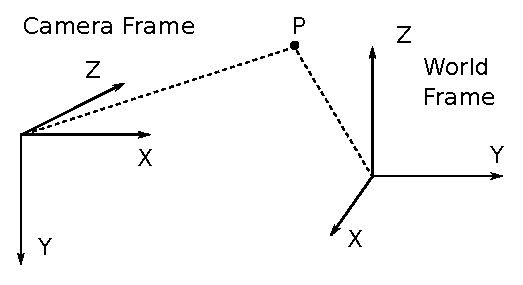
\includegraphics[width=.4\linewidth]{extrinsicparams.eps}
  \caption{Extrinsic parameters}
  \label{fig:pincam_ext}
\end{figure}

The camera's extrinsic parameters are its position and orientation in the 3D world. They are not constant, and change as the camera is displaced.\\

A camera can only take measurements relative to itself, so it makes sense to express the coordinates of 3D points in a coordinate frame relative to the camera. The camera's coordinate frame is defined as follows: the $Z$ direction is defined as pointing out of the camera, and the $X$ and $Y$ directions point towards the right and bottom of the image respectively (see figure \ref{fig:pincam_ext}). This works nicely with image coordinates, where $(0,0)$ is usually defined to be the top-left of the image.\\

However, because the camera will be moving around, points of the map have to be expressed in a reference coordinate system, constant and independent of the movement of the camera. The transformation between the reference coordinate system and the camera's coordinate system defines the camera's extrinsic parameters.\\

Let $p_w = (x_w, y_w, z_w)^T$ and $p_c = (x_c, y_c z_c)^T$ be the coordinates of point $p$ in a reference coordinate system and in the camera coordinate system respectively. Knowing the camera's position and orientation in the reference system, we can deduce the transformation to go from one coordinate system to the other:
\begin{equation}\label{eq:camframe}
  p_c = R \cdot p_w + t
\end{equation}
where $R$ is the rotation matrix between the two coordinate systems, and $t$ is the origin of the reference frame expressed in the camera coordinate system. Using homogenous coordinates, equation \ref{eq:camframe} can be rewritten as follows:
\begin{equation}\label{eq:camframe_bis}
  \begin{bmatrix}
     x_c \\
     y_c \\
     z_c
   \end{bmatrix}
     = [R|t]
   \begin{bmatrix}
      x_w \\
      y_w \\
      z_w \\
      1
   \end{bmatrix}
\end{equation}

The extrinsic parameters of the camera are its position, $t$, which has three degrees of freedom, as well as its orientation, represented by $R$, which also has three degrees of freedom. The orientation's degrees of freedom can be parametrized as three angles, for example the roll, pitch and yaw angles. It is possible to recover these angles from the rotation matrix, and vice versa. The task of localization will be to recover the camera's extrinsic parameters, and from these, the pose of the drone.

\subsubsection{Intrinsic Parameters}
\begin{figure}[H]
  \centering
  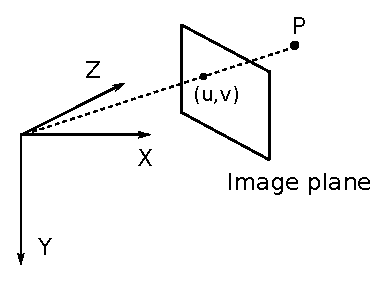
\includegraphics[width=.3\linewidth]{intrinsicparams.eps}
  \caption{Intrinsic parameters}
  \label{fig:pincam_int}
\end{figure}
Once we have the coordinates of point $p$ in the camera's system, we can project this point onto the image plane, using the camera's intrinsic parameters. These are the horizontal and vertical focal lengths $f_x$ and $f_y$, principal point coordinates $c_x$ and $c_y$ and skew factor $s$. From these, the image coordinates $u$ and $v$ can be recovered by projecting the three-dimensional coordinates as follows:
\begin{align}
  u &= \frac{f_xx_c + sy_c}{z_c} + c_x\\
  v &= \frac{f_yy_c}{z_c} + c_y
\end{align}
We can already see that our camera only gives information up to a scale factor, as multiplying all camera frame coordinates by a scalar gives the same image coordinates. The above equations can also we rewritten in matrix form, again using homogenous coordinates:
\begin{equation}
  z_c \begin{pmatrix} u\\v\\1 \end{pmatrix} =
  \begin{bmatrix}
  f_x & s   & c_x \\
  0   & f_y & c_y \\
  0   & 0   & 1
  \end{bmatrix} \begin{pmatrix} x_c\\y_c\\z_c \end{pmatrix}
\end{equation}
The matrix containing all intrinsic parameters of the camera is called the intrinsic matrix $K$:
\begin{equation}
  K = \begin{bmatrix}
  f_x & s   & c_x \\
  0   & f_y & c_y \\
  0   & 0   & 1
\end{bmatrix}
\end{equation}
The intrinsic parameters of the camera can be calculated from the output of the camera through a process called camera calibration. As their name implies, they are characteristics intrinsic to a camera, and do not change during operation, so they only need to be calculated once to be useable as known quantities.\\

Finally, the full projection from world coordinates to image coordinates can be performed as follows:
\begin{equation}
  z_c\begin{pmatrix} u\\v\\1\end{pmatrix} =
    K[R|t]\begin{pmatrix} x_w\\y_w\\z_w\\1\end{pmatrix}
\end{equation}
The projection matrix $P = K[R|t]$ gives the image coordinates up to a scale factor ($z_c$), but this can easily be resolved by normalizing the homogenous image coordinates so that the last coordinate is 1.

\subsection{Lens Distortion}
The pinhole camera model does not perfectly describe the projection of the world onto the camera's image, however, as it neglects lens distortion. Real cameras use lenses, and these lenses slightly deflect the light rays moving through them, so it is not accurate to consider that light travels in a straight line though a pinhole. This deflection causes distortion in the image. We consider two types of distortion: radial and tangential distortion. This distortion can be modeled using the Brown-Conrady distortion model (using a third order approximation for the radial distortion, and a second order approximation for the tangential distortion):
\begin{align}
	x_d &= x_u(1+k_1r^2+k_2r^4 + k_3r^6) + 2p_1x_uy_u + p_2(r^2 + 2x_u) \label{eq:dist1}\\
	y_d &= y_u(1+k_1r^2+k_2r^4 + k_3r^6) + 2p_2x_uy_u + p_1(r^2 + 2y_u) \label{eq:dist2}
\end{align}
Where $k_i$ and $p_i$ are the radial and tangential distortion coefficients respectively, $(x_d,y_d)$ is the distorted image point (where it is actually observed), $(x_u,y_u)$ is the undistorted image point (where it would be observed if there was no distortion), and $r = \sqrt{(x_u - x_c)^2 + (y_u - y_c)^2}$ is the distance between the undistorted point, and the image center $(x_c, y_c)$.  \\
If we know $(k_1,k_2,k_3,p_1,p_2)$, we can invert equations \ref{eq:dist1} and \ref{eq:dist2} to obtain the undistorted points. \cite{opencvcamcalib}

\subsection{Camera calibration}
Both the distortion coefficients and the camera matrix (consisting of the focal lengths, principal point, and skew factor) are intrinsic to the camera. It would be useful to know them once and for all, as they do not change during operation.\\

The process of camera calibration refers to the estimation of the distortion coefficients and camera matrix. It is typically done by looking at checkerboards placed at various points in the camera's field of view. The distortion coefficients are optimized such that the corners on the checkerboards appear on straight lines. The fact that the points of the checkerboard are part of the same plane, and that they form squares is used to estimate the camera's intrinsic parameters. There is a convenient ROS node called \texttt{camera\_calibration} that does this.\\

To be able to use the pinhole camera model in all our algorithms, we will use another convenient ROS node called \texttt{image\_proc} that takes a stream of distorted images as input, and uses the distortion coefficients that were previously estimated to produce a stream of undistorted images as output.

\section{Scale-space representation}
One of the problems when trying to recognize points from a variety of viewpoints, is that depending on the distance between the point and the camera, the point can have many different sizes in the image. The scale-space representation is an attempt to solve this problem. An image can be represented as a two variable function $f(x,y)$, where the value of $f$ is the intensity of the pixel at location $(x,y)$. The scale-space representation of $f$ is a family of signals obtained by convoluting the original signal with a Gaussian filter $g$: $L(x,y;\sigma) = g(x,y;\sigma) \star f(x,y)$. For different values of the parameter $\sigma$ (the scale), the result is a blurred image where finer and finer details are indistinguishable. When $\sigma=0$, the Gaussian becomes an impulse function and the result of the convolution is the original image. The scale-space representation of an image, $L(x,y,\sigma)$ can be seen as a three dimensional image, made by stacking images obtained by blurring the source image more and more. By working on the scale-space representation of images, we ensure that our methods are scale invariant. \cite{scalespace}\\

To illustrate this with an example, we look at figure \ref{fig:scalespace}. Images \ref{fig:scalespace_faraway} and \ref{fig:scalespace_closeby} have been observed and we would like to match them. Zooming in on image \ref{fig:scalespace_faraway} gives \ref{fig:scalespace_faraway_zoomedin}, but this image is quite different from \ref{fig:scalespace_closeby}. If we look at the scale-space representation of \ref{fig:scalespace_closeby} we might find a match at higher scales, when the image becomes blurred to look like image \ref{fig:scalespace_closeby_blurred}. Note that we are matching individual keypoints, which are usually smaller than this image (the corners of this image could each be keypoints).

\begin{figure}[H]
\centering
\begin{subfigure}{.4\textwidth}
  \centering
  \includegraphics[width=.9\linewidth]{scalespace_faraway.png}
  \caption{View from far away.}
  \label{fig:scalespace_faraway}
\end{subfigure}%
\begin{subfigure}{.4\textwidth}
  \centering
  \includegraphics[width=.9\linewidth]{scalespace_closeby.png}
  \caption{View from close by.}
  \label{fig:scalespace_closeby}
\end{subfigure} \\
\begin{subfigure}{.4\textwidth}
  \centering
  \includegraphics[width=.9\linewidth]{scalespace_faraway_zoomedin.png}
  \caption{From far away, zoomed in.}
  \label{fig:scalespace_faraway_zoomedin}
\end{subfigure}%
\begin{subfigure}{.4\textwidth}
  \centering
  \includegraphics[width=.9\linewidth]{scalespace_closeby_blurred.png}
  \caption{From close by, filtered by a Gaussian.}
  \label{fig:scalespace_closeby_blurred}
\end{subfigure}
\caption{Usefulness of the scale-space representation.}
\label{fig:scalespace}
\end{figure}

\section{SURF Keypoint Detector}
The SURF detector uses the determinant of the Hessian matrix to measure local change around points. The Hessian matrix is defined as follows:
\begin{equation}
  \mathcal{H}(\bf{x},\sigma) =  \begin{bmatrix}
  L_{xx}(\bf{x},\sigma) & L_{xy}(\bf{x},\sigma)\\
  L_{xy}(\bf{x},\sigma) & L_{yy}(\bf{x},\sigma)
\end{bmatrix}
\end{equation}
where $L_{xx}$, $L_{xy}$ and $L_{yy}$ are the convolution of the image with the second order derivatives of the Gaussian $g(\bf{x};\sigma)$. The creators of SURF decided to approximate the second order Gaussian derivatives with box filters. This decision stemmed from the fact that even though Gaussian filters are optimal, they are already modified quite heavily, as they have to be discretized and cropped, and the result of the convolution is then resampled. The big advantage of using square filters is that they can be evaluated very quickly by using integral images. To obtain a scale-space representation, the SURF method uses box filters of different sizes: for example, a 9x9 filter, approximates a Gaussian with parameter $\sigma = 1.2$, with larger filters corresponding to bigger values of $\sigma$. Local maxima on 3x3x3 neighborhoods of the scale-space representation are then taken as points of interest.\\

Finally, so that the detected keypoints are rotationally invariant, we need to assign an orientation to each keypoint that can be recognized from subsequent viewpoints. To do this, the SURF method computes the response to vertical and horizontal Haar wavelets in a circular neighborhood of radius $6s$ around the detected points, $s$ being the scale at which that point was detected. The Haar wavelets are rectangle shaped, so their response can also be computed efficiently using integral images. The responses are plotted in a plane, where the abscissa is the horizontal response, and the ordinate is the vertical response. The responses are summed within a sliding orientation window, giving an orientation vector for each position of the sliding window. The orientation vector with the largest norm is taken to be the orientation of the keypoint.
\cite{surf}

\section{SIFT Keypoint Descriptor}
\begin{figure}[H]
  \centering
  \includegraphics[width=\textwidth]{siftdescriptor.png}
    \caption{Illustration of a SIFT descriptor. Each subregion containing 4x4 points defines a histogram with 8 bins. Note that SIFT uses 4x4 subregions, not 2x2 like in this illustration. \cite{sift2}}
    \label{fig:siftdescriptor}
\end{figure}
To create a SIFT descriptor, a 16x16 square region is taken around the keypoint. This region is rotated and scaled according to the orientation and scale of the detected keypoint. The 16x16 region is subdivided into 16 4x4 subregions. In each subregion, a histogram of local gradients is computed and quantized into 8 bins. The magnitudes of these histograms form the descriptor. Figure \ref{fig:siftdescriptor} shows an illustration of the histograms. As there are 16 histograms of 8 bins each, the total length of the descriptor vector is 128. \cite{sift}

\subsection{Limitations}
The dimension of SIFT descriptors is 128, which is quite large. Having such a large dimension has the advantage of allowing the descriptors to be highly discriminative, even with many different keypoints, but the disadvantage of requiring more space to be saved, and to slow down the matching algorithms that will be used later on.\\

Another limitation is that the points detected are points of the image with a high intensity gradient. These points are often corners, with two distinctive regions, one inside and one outside the corner. The descriptor depends on the gradients of the image, which depend on both these regions. To be able to recognize the keypoints, the descriptors have to be similar independently of the viewpoint of the keypoint. This is the case when both regions of the corner are part of the same plane, like in the case of a 2D drawing, but it is not the case when the inside of the corner is some object, and the outside is the background, as the background can change depending on the viewpoint. For example, figure \ref{fig:siftlimit} shows the same point seen from two different angles, where the descriptor would be quite different, because there is a different background
\begin{figure}[H]
\centering
\begin{subfigure}{.4\textwidth}
  \centering
  \includegraphics[width=.9\linewidth]{siftlimit1.png}
\end{subfigure}%
\begin{subfigure}{.4\textwidth}
  \centering
  \includegraphics[width=.9\linewidth]{siftlimit2.png}
\end{subfigure} \\
\caption{Two views of a same point, with a different background.}
\label{fig:siftlimit}
\end{figure}

\section{Keypoint Tracking}
Because the above algorithm to extract a descriptor of a keypoint is quite slow (it takes approximately \SI{413}{\milli\second} to extract all descriptors from a new image, see table \ref{tab:cvtime}), it is not practical to run these algorithms on each new image, as this would greatly reduce the frame rate. For this reason, another, faster alternative has been found : keypoint tracking. This method finds keypoints by looking for keypoints that were observed in the previous image, and assuming that their displacement inside the image was small. \\

The algorithm used for this keypoint tracking is called the pyramidal Lucas-Kanade method \cite{pyramidallucaskanade}. This method assumes that the movement between successive frames is small and can be approximated by an affine transformation in local regions. It uses small dense pixel regions to estimate the movement of a keypoint between successive frames. The method was explained more in detail in last year's master thesis \cite{jacquesleclere}.\\

Keypoint tracking has the advantage of being much faster than detecting new keypoints, especially because the descriptor of each tracked keypoint is already known and does not have to be extracted again at each frame. The main drawback of this method is that it does not allow to detect any new keypoints, as all tracked keypoints have to be present in the previous frame.

\section{Detection and Tracking hybrid}

In the previous years, detection and tracking were used alternatively: each new frame was populated with keypoints using one of the two methods. As long as there were enough keypoints in the preceding frame, tracking was used on all these keypoints with no detection of new keypoints. While tracking is used, the number of keypoints in each successive frame is non-increasing, as each keypoint can either be lost or tracked, and when the number of keypoints in the frame fell below some threshold, keypoint detection was used to populate the next frame with new keypoints.\\

When the detection method is used, all previous keypoints are discarded, and keypoints are detected on the entire image. The reason for this choice was that detection was too slow to be used on each frame, but necessary to find new keypoints, and that if detection and tracking were used simultaneously, keypoints that are already being tracked would be re-detected, which would result in duplicate keypoints in the same frame. However, this method is suboptimal, because every time detection is used, all currently tracked keypoints are lost and have to be re-detected. It also causes quite an inconsistent frame rate.\\

\begin{figure}[H]
  \centering
  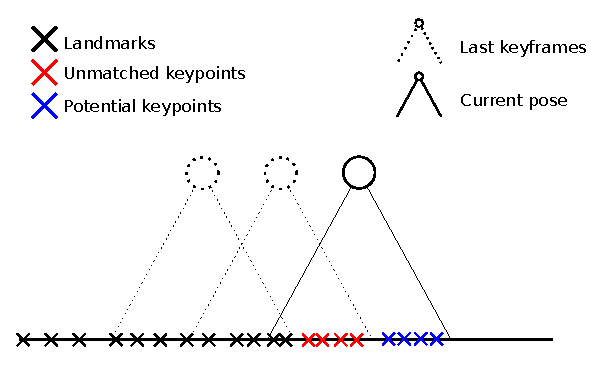
\includegraphics{keyframe_landmark_illustration.eps}
  \caption{Delay between first observation of a keypoint, and mapping of this keypoint.}
  \label{fig:delay}
\end{figure}

In addition to being suboptimal, this method has a few drawbacks that make it hard to use for this project. As we will see later, at least two views of a single keypoint from different keyframes are required to estimate the 3D position of the corresponding landmark. Figure \ref{fig:delay} is an illustration of this problem, in a one dimensional world. When a keypoint is seen for the first time and saved in a keyframe, it becomes an unmatched keypoint (red cross), and its 3D location is unknown. It has to be observed from a second keyframe in order to become a landmark (black cross), with an estimated 3D position. Only then can it be used as a reference to localize the drone.\\

On figure \ref{fig:delay}, if the drone creates a new keyframe at its current position, the unmatched keypoints can become landmarks, and the potential keypoints (blue crosses) become new unmatched keypoints. If we had only used tracking since the last keyframe, however, we would not have detected those potential keypoints. As a result, when the drone continues advancing it would not have any unmatched keypoints from the previous keyframe, and it would not be able to add any landmarks to the map. The difficulty lies in the fact that each time we create a new keyframe, we ideally need to see:

\begin{enumerate}
\item Enough already mapped landmarks to accurately estimate the position of the new keyframe
\item Unmatched keypoints from previous keyframes so that we can put them into the map to allow further exploration
\item New, previously unobserved keypoints to ensure long-term viability (these points will be the unmatched keypoints of the next keyframe)
\end{enumerate}

The need for these three ingredients means that keyframes have to be created more frequently than when we are mapping keypoints from single observations. In many cases, there are enough common keypoints between successive keyframes so that the old method did not require detection at any moment between the two keyframes. As a result, all keypoints of the most recent keyframe would already have been observed before. This means that they can be added to the map, but it seriously harms possible future exploration, as the third element of the above list is missing, so it won't be able to create any new landmarks when the next keyframe is created. Simply decreasing the threshold at which we used detection instead of tracking was not a good solution as it resulted in many more slow detection steps.\\

To solve this problem, a new technique had to be found. It is clear that we need new, unmatched keypoints in each keyframe, and these points cannot be tracked from previous images, so they have to be detected. However, keypoint detection takes so much time it's prohibitive to do it on each image. We noticed that the vast majority of keypoints that are lost during tracking are lost because they are moved out of the field of vision, so they leave the image from the sides. Similarly, new potential keypoints enter the field of view from the sides, so after some displacements, there will often be sections of the image with many keypoints (parts of the scene that were observed continuously since the last full keypoint detection), and sections of the image with no keypoints (parts of the scene that were not in the field of view when the last full detection took place). Our solution is to treat the part of the image with no keypoints as if it was a separate image, and do keypoint detection on that part, while keeping the part of the image with keypoints, and tracking its keypoints. This is illustrated on figure \ref{fig:trackdetecthybrid}.

\begin{figure}[H]
\centering
\begin{subfigure}{.33\textwidth}
  \centering
  \includegraphics[width=.9\linewidth]{track_detect_hybrid_start.png}
  \caption{Initial frame}
  \label{fig:trackdetecthybrid_a}
\end{subfigure}%
\begin{subfigure}{.33\textwidth}
  \centering
  \includegraphics[width=.9\linewidth]{track_detect_hybrid_mid.png}
  \caption{After displacement and tracking}
  \label{fig:trackdetecthybrid_b}
\end{subfigure}
\begin{subfigure}{.33\textwidth}
  \centering
  \includegraphics[width=.9\linewidth]{track_detect_hybrid_end.png}
  \caption{After detection}
  \label{fig:trackdetecthybrid_c}
\end{subfigure}
\caption{Illustration of the hybrid between tracking and detection.}
\label{fig:trackdetecthybrid}
\end{figure}

We can see on table \ref{tab:cvtime} that our hybrid method takes about \SI{55}{\milli\second} per image. This is the time for both the tracking of the keypoints of the previous image, and detection and description of keypoints on the sides. Ideally, we would like this time to be below \SI{33}{\milli\second}, because our front camera has a rate of 30 FPS, so it sends an image every \SI{33}{\milli\second}. However, we do not need to use our hybrid at every new image, only when a significant part of the sides of the image contains no points from tracking. The rest of the time, we can use pure tracking, which runs in \SI{6}{\milli\second}. In the end we are alternating between tracking and our hybrid method, instead of between tracking and full detection. The end result is that we are more regular, both in the number of keypoints of any given frame, and in the computation time required per frame.

\begin{table}[H]
  \centering
  \small\addtolength{\tabcolsep}{-2pt}
  \sisetup{round-mode=places, round-precision = 3}
  \begin{tabular}{ @{} l @{\hspace{10mm}}     S[table-format=3.0] @{}  }
    \toprule
    Task & \multicolumn{1}{l}{Time per Frame [\si{second}[]}  \\
    \midrule
    Keypoint detection   & \num{0.032} \\
    Keypoint description & \num{0.413} \\
    Keypoint tracking    & \num{0.006} \\
    Hybrid               & \num{0.055} \\
    \bottomrule
  \end{tabular}
  \caption{Timings for the different tasks. The time for the hybrid method includes tracking, detection, and description.}
  \label{tab:cvtime}
\end{table}
\newpage
\section{Keypoint Matching}
The final computer vision task is keypoint matching. After keypoints from multiple viewpoints are saved, we need to know which observations correspond to the same point. This is needed when a keyframe is added to the map, because we need keypoint matches to place landmarks in the map, and also when trying to match an image with the map to localize the drone. We will compare the descriptors of the keypoints to determine which ones are similar enough to represent the same point. The Euclidean distance is a good metric of how different the descriptors are, because they are vectors of floating point numbers (if we were working with binary descriptors, like in the case of BRIEF, we should use the Hamming distance instead).\\

When matching a query image with a reference image, we find the nearest descriptor of the reference image for each descriptor of the query image. For each pair, we then determine if they are close enough to be considered a match. Finding the exact nearest neighbor would take $O(n*m)$ time for an exhaustive search, where $n$ and $m$ are respectively the number of keypoints in the query and in the reference images. A search with a k-d tree runs in $O(n\log(m))$ time, but suffers from the curse of dimensionality, so in high dimensional spaces it is not always faster than an exhaustive search in practice.\\

To overcome these problems, we only look for an approximate nearest neighbor. There exist many different approximate nearest neighbor methods, one of the most famous for high dimensional search is the best-bin first method, which was recommended by the creators of SIFT. It is based on a k-d tree and finds the nearest neighbor in most cases, and a very close neighbor the rest of the time. Other, better approximate nearest neighbor methods have since been invented, so to marginalize the choice of an approximate nearest neighbor algorithm, we use the implementation of a FLANN matcher of OpenCV for the nearest neighbor computation. FLANN stands for Fast Library for Approximate Nearest Neighbors. It contains many state-of-the-art nearest neighbors algorithms and automatically chooses the most appropriate one depending on the data. It is quite fast: to find amongst $666$ keypoints of a keyframe the closest match for each of $502$ keypoints of another keyframe, it took approximately \SI{21}{\milli\second}.

\section{Summary}
In the code, the computer vision node serves as an intermediary between the output of the camera and the input of the localization and mapping nodes. It transforms each image into a list of keypoints, each with their 2-dimension location on the image plane, and 128-dimension descriptor. To do this, it first undistorts the image, using distortion coefficients estimated in advance, then either tracks keypoints from the previous frame, and detects descriptors at the edges of the frame, or discards all keypoints of the previous frame and detects keypoints on the entire image. In both cases, descriptors for the newly detected keypoints are then extracted. Later, the localization and the mapping nodes can use keypoint matching to find keypoints in different frames that correspond to the same landmark.\\

In this part, we kept using SIFT descriptors and a SURF detector, as was implemented last year, but the OpenCV library contains procedures for working with many other types of descriptors and detectors, which were not tested this year. In future work on this project, it might be interesting to test using other types of keypoints, such as ORB, as the tests leading to the choice for the current SIFT/SURF combination were made before the current 3D framework existed.\\
Figure \ref{fig:cvflowchart} summarizes the computer vision part of the code in the form of a flowchart.

\begin{figure}[H]
\centering
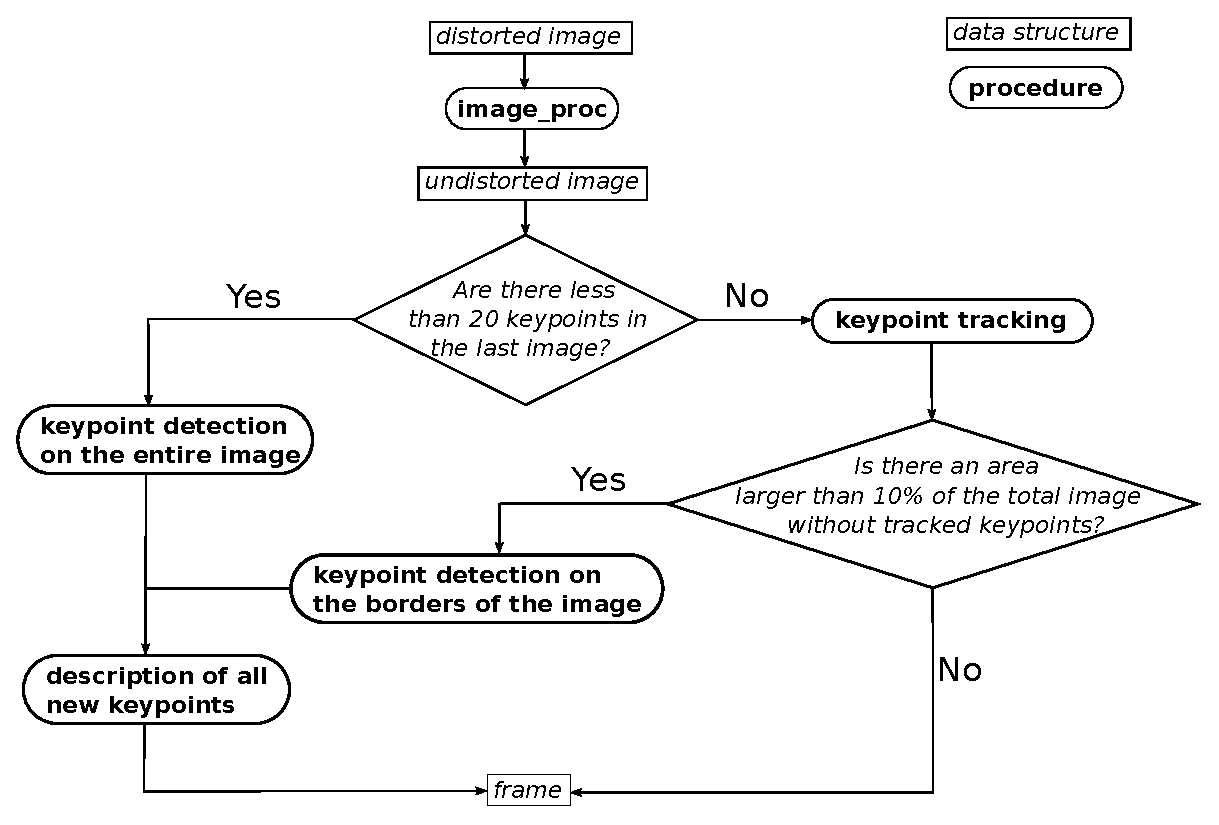
\includegraphics[width=\linewidth]{cvflowchart.eps}
\caption{Flowchart of computer vision node}
\label{fig:cvflowchart}
\end{figure}


\chapter{Localization} %5
%%Localization (chpt4)
The first of the two main ingredients of SLAM is localization. The task of localization is the estimation of the drone's position given a map and sensor information. In our case, the map is a map of visual features, and the main sensor used will be the camera. This part was already carried out by last year's groups, and it is already made to work in the three dimensional case. For completeness, we quickly repeat in this chapter how it works.\\

\section{Perspective-$n$-Point}
To localize the drone using visual information and a map, we need to solve the perspective-$n$-point (PnP) problem. PnP is the problem of estimating the six degrees of freedom 3D pose of a camera, given $n$ observations of 3D points whose locations are known. We use two main methods to solve the PnP problem: P3P and EPnP.\\

\subsection{P3P}
The smallest number of point correspondences required to solve the PnP problem is 3, in which case it is called P3P. P3P can be solved with a method based on the cosine law, but it can have multiple solutions. A fourth point correspondence can be used to solve this uncertainty. Given three known points $A$, $B$ and $C$, and the center of projection of the camera $P$, define the following distances: $|A B| = c'$, $|B C| = a'$, $|C A| = b'$, $|P A| = X$, $|P B| = Y$, $|P C| = Z$, and the following angles: $\widehat{APB} = \alpha$, $\widehat{BPC} = \beta$, $\widehat{CPA} = \gamma$. We can then use the cosine law on each of the triangles that has $P$ and two of the points $A$, $B$, $C$ as vertices to obtain the following system of equations:
\begin{align}
  X^2 + Y^2 - XY\cdot2\cos(\alpha) - c'^2 &= 0 \\
  Y^2 + Z^2 - YZ\cdot2\cos(\beta)  - a'^2 &= 0 \\
  Z^2 + X^2 - ZX\cdot2\cos(\gamma) - b'^2 &= 0
\end{align}
The only unknowns is these equations are $X$, $Y$ and $Z$, as the distances between points $A$, $B$, $C$ can be deduced from their known position, and the angles can be deduced from the observations of these points on the image. For the resolution of these equations, the reader is referred to the paper that established the P3P method \cite{p3p}. As they show, it is possible to eliminate one of these equations and one of the variables to end up with two quadratic equations and two unknowns. This means that is there exists a finite number of solutions, that number has to be less than or equal to 4. To eliminate the bad solutions, we can use a fourth point correspondence. Once $X$, $Y$ and $Z$ are determined, the position and orientation of point $P$ be can be deduced.

\subsection{EPnP}
EPnP (Efficient PnP) \cite{epnp} is a method to solve the more general PnP problem. It uses $n \geq 4$ point correspondences to estimate the position of the camera. The central idea of this method is to express the $n$ points as a weighted sum of four virtual points. Because it uses more points, it is be more stable and resistant to noise than P3P.

\subsection{Random Sample Consensus}
Our data is subject to noise and measurement errors, which can negatively impact our solution. Do deal with this problem, we use Random Sample Consensus (RANSAC). RANSAC is a method to estimate parameters using data that contains outliers. The general idea is to iteratively estimate the parameters using different random samples, and to use a voting scheme to select the best parameters. The algorithm works in two steps:
\begin{enumerate}
  \item A random sample is drawn from the data with the smallest number of examples to estimate model parameters. From this random sample, we estimate the parameters.
  \item We test all the data against the model estimated in step 1. All the data that whose loss according to some predefined loss function falls below a certain threshold when fitted to the model is considered part of the consensus set.
\end{enumerate}
Both above steps are repeated, and the model with the largest consensus set is selected. All the data that are part of this consensus set are considered to be inliers, and the rest of the data are considered outliers. A final model can then be computed using all inliers \cite{ransac}.\\
Applying this scheme to the PnP problem, we use the P3P method to create a model from each of the random samples, and then use the EPnP method on the inliers. This way we determine what points are outliers with the fastest method (P3P), and then use EPnP so that all inliers are used for the final estimation.

\section{Visual Odometry from optical flow}
Using the output of the bottom-facing camera, it is possible to deduce the ground speed of the drone. Because monocular camera measurements always give information only up to a scale factor, this only gives the ratio between altitude and speed. However, using the ultrasound sensor, that also points downwards, we know the altitude of the drone and can deduce its absolute ground speed. This visual odometry is already implemented by the constructor of the drone, as it is used to control the velocity of the drone during normal (remote-controlled) use. Unfortunately, the code that computes this velocity from the optical flow is a black box inside the closed-source firmware, so we only have access to its output. Those speed estimations can then be integrated to obtain an estimation of the displacement.\\


\section{Pose Fusion}\label{sec:posefusion}


\chapter{Mapping} %10
%% Mapping (chpt5)
The task of mapping was the main challenge of this work. This task consists in placing recognizable features in a map, that can later be used as landmarks by the drone to estimate its own position. The main challenge in the 3D case, is that a point needs to be observed from at least 2 different positions to be mapped. The simplest approach to map a point, is to simply triangulate its position from two different views. We will begin by exploring this approach. We will find that although this does work reasonably well when we are certain of the position of the cameras, it does not when this position is uncertain. In addition, this method does not allow to take more than two views into account. To remedy these problems we will implement a bundle adjustment step, that allows to build a map that is globally consistent. Throughout this section, we will have to make design choices to try to obtain a method that is both fast enough to work in real time, and accurate enough for the drone to control its position. To evaluate these performances, we will perform a standardized test.

\section{Evaluation procedure} \label{evalproc}
The evaluation will happen in two phases: first the drone will initialize its map and then it will be moved to various known locations, and we will measure the accuracy of its position estimation. The setup used for this evaluation is illustrated on figure \ref{fig:benchmarksetup}. During the initialization phase, we will try to emulate the way the drone would initialize its map just after taking off during a real flight mission (see more in section %TODO
). First the drone is place in a know position on a table (position A in figure \ref{fig:benchmarksetup}). There, the drone is turned on, and it begins initializing its map. The drone is then successively places in 3 other known locations (B, then C, then D), and at each of these locations, the drone in manually communicated its position. Every time this happens, the drone adds landmarks into the map, and optionally updates existing landmarks' position, or even removes some landmarks. In reality, the drone would not know its exact position when taking views at points B, C, and D (position A is defined as the origin), especially at the beginning, as it would have to rely on its IMU and other internal sensors to estimate its position. To emulate this, we implement a second type of test: the robustness test, where the position that is communicated to the drone is slightly different from its real position, at each of the uncertain points (B, C, and D).\\
In the second phase of the evaluation, the drone is again placed at different known locations. This time, no information is communicated to the drone from the outside, and the drone does not modify its map. The drone estimates its position using only its camera and the map that it built during the initialization phase. We compare the drone's estimated position with its real position to evaluate the quality of the map. The two quantities we will seek to optimize are the accuracy of the drone's postition estimation, and the time taken to compute the map.


\begin{figure}[H]
  \centering
  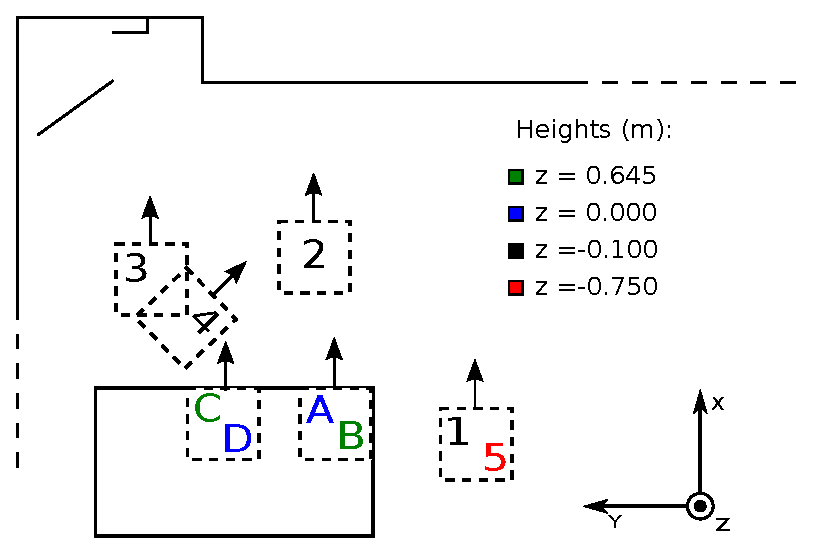
\includegraphics{benchmark_setup.eps}
  \label{fig:benchmarksetup}
  \caption{Different positions of the drone during the validation}
\end{figure}

\subsection{Experimental setup}
We will conduct two different finds of experiments: one to measure the accuracy, and one to measure the robustness of the mapping method. In both cases, we begin by placing the drone at the corner of a desk (position A on figure \ref{fig:benchmarksetup}). After the drone has saved its view, it is placed on a stool exactly above its first position. Its exact pose is then manually communicated to the drone to simulate the measurements from its IMU and ultrasonic sensor. The drone then again takes a snapshot of its camera input, and matches points with the first view, and then adjusts its second pose and the position of the points through bundle adjustment. The drone and stool are then moved to the left (position B on fiugre \ref{fig:benchmarksetup}), and again manually given its exact position, after which it takes another snapshot, matches points with the first two views, and readjusts the poses of the keyframes anf the positions of the points through bundle adjustment. This entire process is rpeated a third time when the drone is placed on the desk again at position D. The initialization of the map consists in making these four keyframes and adjusting their position and that of the landmarks 3 times. After this initialization is done, we place the drone at different locations, and measure how close it is to where it thinks it is. We evaluate the initialization based on how accurate its position estimation is, as well as on how much time the successive bundle adjustments took.


\section{Triangulation}
In the problem of triangulation, we try to find the 3D coordinates of a point from the 2D coordinates of the projection of this point on two images that were seen from different positions. We assume that the position of the camera taking these images is known exactly at both locations. If the camera positions is known exactly, and if the projection of the points into the image planes was perfect, then the two rays going from the camera centers, and through the images of the points would intersect at the location of the 3D point. In practice however, these two rays never cross exactly, so a method has to be found to find the best possible location of a 3D point from the pair of images.

\subsection{Midpoint Method}
The simplest solution would be to take the midpoint of the common perpendicular of the two rays. This method is intuitive to understand geometrically, and is quite easy to compute. In practice, however its results are not very good, as there is no theoretical reason for this point to be the best. The optiaml solution would be to displace the pixels on both images until the resulting rays meet, keeping the displacement of the pixels as small as possible (in the least squared sense). Such a solution would give the maximum likelihood estimator of the position of the 3D points, under the assumption that the error of their projection on the image planes follows gaussian noise.

\subsection{Optimal Correction}
There are several algorithms in the litterature that triangulate the position of a point using optimal correction. The most popular one, proposed by Hartley and Sturm \cite{hartleysturm}, computes the solution directly but requires finding the root of a 6th degree polynomial. Kanantani et. al.'s method \cite{kanatani} finds a solution iteratively, but requires very few iterations to have an accurate solution, and in practice, is faster than the Hartley Strum method. It also has better numerical properties, as unlike the Hartley-Sturm method, it does not have singularities at the epipoles.

\subsection{Comparison of triangulation methods}
Using the evaluation procedure described in section \ref{evalproc}, we can compare these 2 triangulation methods.

\begin{table}[H]
  \centering
  \caption{Comparison between triangulation methods}
  \small\addtolength{\tabcolsep}{-2pt}
  \sisetup{round-mode=places, round-precision = 3}
  \begin{tabular}{ @{} l S[table-format=2.3] S[table-format=2.3] S[table-format=2.3] S[table-format=2.3] S[table-format=2.3] @{}  }
    \toprule
    {}                 & \multicolumn{2}{c}{Accuracy} &  \multicolumn{2}{c}{Robustness} &   \multirow{2}{4em}{Computation Time (\si{\second})} \\
    {}                 & {\footnotesize Distance (\si{\meter})} & {\footnotesize Angle (\si{\radian})}
    & {\footnotesize Distance (\si{\meter})} & {\footnotesize Angle (\si{\radian})} &   \\
    \midrule
    Midpoint Method    & \num{0.121729436669}  & \num{0.052339119893} & \num{0.844616151792} & \num{0.27019708855} & \num{0.012}\\
    Optimal Correction & \num{0.0988557438948} & \num{0.0406436455673}& \num{0.775954169079} & \num{0.218538344815}& \num{0.024}\\
      \bottomrule
  \end{tabular}
  \label{fig:triangcompare}
\end{table}


The computations were timed during the accuracy test, but these timings should be the same for the robustness tests. %TODO justify this
We can see that the optimal correction method is more performant, at the cost of being computationally heavier. We will see, however, that this computation time is negligible in comparison with the time taken for bundle adjustment. Therefore, we will use the optimal correction method to triangulate points.

\section{Bundle Adjustment}
Unfortunately the main source of errors when mapping points is not inaccuracy of the camera, but uncertainty on the camera's position. This is bad, as a bad estimation of the camera's position will result in badly located landmarks, which in turn will result in a bad estimation of the camera position. In the long term, errors will accumulate, and the map will be completely distorted. Luckily, if we have enough point correspondences between two images, it is possible to deduce the relative displacement between the two images. This means that from a set of images, we can reconstruct a scene, without even needing a prior estimation of the position of the cameras that took the images. This is good news as it means that the images can give us some absolute information about the scene, not only relative to the drone. The problem of adjusting camera positions and 3D point locations in order to minimize the reprojection errors of the 3D points onto the image planes is known as bundle adjustment. As stated above, bundle adjustment has the advantage of being absolute with respect to the world, and so not having errors accumulate. Another advantage of bundle adjustment, is that it can easily take into account points that are seen by more than two cameras, which is not trivial for the triangulation techniqhes described above. The main disadvantage of bundle adjustment is that it is computationally heavy, so it is important to adapt it to be useable un real time.\\
To show the advantages of bundle adjustment, we compare it with triangulation using the optimal correction method. When using bundle adjustment, optimal correction triangulation is also used to obtain an initial solution, from which we optimize.


\begin{table}[H]
  \centering
  \caption{Performance of Bundle Adjustment}
  \small\addtolength{\tabcolsep}{-2pt}
  \sisetup{round-mode=places, round-precision = 3}
  \begin{tabular}{ @{} l S[table-format=1.3] S[table-format=1.3] S[table-format=2.3] S[table-format=1.3] S[table-format=1.3] S[table-format=2.3] @{}  }
    \toprule
    {}      & \multicolumn{3}{c}{Accuracy} &  \multicolumn{3}{c}{Robustness} \\
    {}      & {\scriptsize Distance (\si{\meter})} & {\scriptsize Angle (\si{\radian})} & {\scriptsize Time (\si{\second})}
            & {\scriptsize Distance (\si{\meter})} & {\scriptsize Angle (\si{\radian})} & {\scriptsize Time (\si{\second})} \\
    \midrule
    No Bundle Adjustment  &\num{0.0988557438948}&\num{0.0406436455673}&  {\textemdash}    &\num{0.775954169079}&\num{0.218538344815}&  {\textemdash}      \\
    With Bundle Adjustment&\num{0.0897626230568}&\num{0.029930165598} &\num{15.7027562261}&\num{1.37414105299} &\num{0.492183127143}&\num{13.8024009466}  \\
    \bottomrule
  \end{tabular}
  \label{fig:bacompare2}
\end{table}


We see that in the accuracy test, bundle adjustment gives a significant improvement to the performance of the pose estimation. In the robusteness test, however, bundle adjustment makes the results quite worse. This is surprising, as it is just in the case where the pose of the camera is uncertain that bundle adjustment should improve de result, by adjusting the pose of the camera. But because the problem is quite non linear, it is possible to fall in local minima. We will later see that by tuning the bundle adjustment phase, we can make it perform much better, and actually improve the results in the robustness test. The other big problem of bundle adjustment is the time it takes. In both tests, this time was over \SI{13}{\second}, which is a prohibitively large amount of time for real time applications. In addition to improving the performance on the robustness test, we will try to recude the time taken by the bundle adjustment.

\section{Tuning the Bundle Adjustment}
The main drawback of Bundle Adjustment is that it requires an iterative method to be solved and can take a lot of time, which of course is a limiting factor for a robot that builds a map in real time. Therefore it is important to optimize both the speed of the computations, and their accuracy. As is often the case, there will have to be a tradeoff between these two. To measure both the speed of the Bundle Adjustment and the accuracy of the map obtained, we will conduct some experiments using different parameters to initialize the map.

\subsection{Convergence of the solver}
The first element we can tune is the convergence criterion of the solver that solves the bundle adjustment problem. We will stop when the ratio of the change in the objective function to the value of this function arrives below some threshold. This ensures that the criterion scales with the problem, which is important as the size of the problem can vary during operation (as the map grows, for example). The default value of the Ceres solver is $10^{-6}$, but experimentally, we find that we can use a softer threshold to significantly speed up the computations, without impactig the quality of the results too much (and even improving them in the robustness test).

\begin{table}[H]
  \centering
  \caption{Effect of convergence criterion on Bundle Adjustment speed and performance}
  \small\addtolength{\tabcolsep}{-2pt}
  \sisetup{round-mode=places, round-precision = 3}
  \begin{tabular}{ @{} S[scientific-notation=true] S[table-format=1.3] S[table-format=1.3] S[table-format=2.3]
                                                   S[table-format=1.3] S[table-format=1.3] S[table-format=2.3] @{}  }
    \toprule
    \multirow{2}{4em}{Convergence Threshold}  & \multicolumn{3}{c}{Accuracy} &  \multicolumn{3}{c}{Robustness} \\
        & {\scriptsize Distance (\si{\meter})} & {\scriptsize Angle (\si{\radian})} & {\scriptsize Time (\si{\second})}
        & {\scriptsize Distance (\si{\meter})} & {\scriptsize Angle (\si{\radian})} & {\scriptsize Time (\si{\second})} \\
    \midrule
    \num{10}       &\num{0.0988557438948}&\num{0.0406436455673}&\num{0.528740555048}&\num{0.775553503184}&\num{0.219380944042} &\num{0.527468636632} \\
    \num{5}        &\num{0.0988557438948}&\num{0.0406436455673}&\num{0.532568186522}&\num{0.775954169079}&\num{0.218538344815} &\num{0.560289662331} \\
    \num{1}        &\num{0.0988557438948}&\num{0.0406436455673}&\num{0.536680459976}&\num{0.775954169079}&\num{0.218538344815} &\num{0.529257409275} \\
    \num{0.5}      &\num{0.0988557438948}&\num{0.0406436455673}&\num{0.532132491469}&\num{0.284057820455}&\num{0.0860006110714}&\num{0.61461224407}  \\
    \num{0.1}      &\num{0.116334787731} &\num{0.0370860746263}&\num{0.67120449245} &\num{0.244478011775}&\num{0.0982536795903}&\num{1.17620864138}  \\
    \num{0.05}     &\num{0.0684117396072}&\num{0.01622317801}  &\num{0.742543946952}&\num{0.291411483818}&\num{0.112600996782} &\num{2.11719946936}  \\
    \num{0.01}     &\num{0.0895791917611}&\num{0.032296133528} &\num{1.42051474378} &\num{0.823415005012}&\num{0.316300896325} &\num{2.77009601146}  \\
    \num{0.005}    &\num{0.0908954991063}&\num{0.0308365172421}&\num{1.53279625252} &\num{0.142093947791}&\num{0.0495629729962}&\num{4.18590991944}  \\
    \num{0.001}    &\num{0.0849543195902}&\num{0.023134969351} &\num{3.61956872419} &\num{1.034983532}   &\num{0.397193935917} &\num{4.90690393746}  \\
    \num{0.0001}   &\num{0.0842253035954}&\num{0.0258716997751}&\num{5.05812323838} &\num{1.36150222356} &\num{0.479872553731} &\num{10.4840388894}  \\
    \num{0.00001}  &\num{0.0899028376206}&\num{0.0299204957695}&\num{12.4531462789} &\num{1.4834446381}  &\num{0.528430316164} &\num{13.2059885859}  \\
    \num{0.000001} &\num{0.0897626230568}&\num{0.029930165598} &\num{15.7027562261} &\num{1.37414105299} &\num{0.492183127143} &\num{13.8024009466}  \\
    \num{0.0000001}&\num{0.0875171189566}&\num{0.0282118025117}&\num{15.7951563597} &\num{1.55886341652} &\num{0.567309620599} &\num{12.934817493}   \\
    \bottomrule
  \end{tabular}
  \label{tab:convergencetol}
\end{table}

As we can observe on table \ref{tab:convergencetol}, the more severe the convergence threshold, the better the performance on the accuracy test. On the robusteness test, however, this is true for high convergence thresholds, but when the convergence threshold is lower than \num{0.01}, the performance starts to degrade as the convergence threshold becomes lower. In both the accuracy and robustness tests, the lower the threshold, the longer it takes. We will chose a threshold of \num{0.05}, as it is a nice compromize of performance on the accuracy test, performance on the robustness test, and speed.

\subsection{Rejecting outliers}
When looking closer at the results of bundle adjustment, we find that a large part of the errors come from a small number of points. One possible explanation is that these points do not correspond to real world points, so that even if we have the correct position of all cameras exatly, the rays corresponding to these points will not intersect, or even be close to intersection. For this reason, after every bundle adjustment pass, we could look at the contribution of every mapped point to the objective function, and eliminate points whose error is too high. Before doing this we have to take some things into account that as a point is observed by an increasingly large number of cameras:
\begin{itemize}
  \item Its total contribution to the cost function will increase, as each observtion of a point adds a term to the objective funtion
  \item Its contribution per observation to the cost function will also increase, because every time an observation is added, the location of the point will change a bit, and its position will become less optimal if we only consider the cameras that already saw the point before.
\end{itemize}
For these reasons, we will put a different threshold on the points depending on the number of cameras that see the point. If a point is seen by a large number of cameras, we will allow it to have larger errors in the objective function before removing it.











\section{Map Initialization}
A robot needs a map lo localize itself within it, but it needs to know its position to find the postion of surrounding objects and build a map. Because the mapping and localization tasks are mutually dependent on one another, there needs to be a special procedure to build a map from nothing when it does not exist yet. Arbitrarily, we decide that the position of the drone when it starts flying is the origin (in all 6 degrees of freedom) of the map. However, with only a monocular camera, it is not possible to find the exact location of any visual features from one observation only, views from at least two different positions are needed to triangulate points.


%%blabla

To reach the position from which the drone will take a second view and triangulate points, the drone has to fly blindly. Blindly here means without using a map la localize itself visually, but the drone can still use its other sensors (IMU and ultrasonic sensor) to obtain an estimate of its postion. Because the ultrasonic sensor is much more accurate than the IMU, and gives an absolute measure, we will mostly rely on this sensor to estimate the relative position from where we take the second view. Because the ultrasonic sensor only gives the distance from the bottom of the drone to the ground, the drone should fly straight up from its first position (the origin) to reach its second position.\\
Once in its second position, the drone can match seen keypoints from both views, and from its estimated position, triangulate those points to the map. However, the drone's estimation of its pose is prone to errors, especially as it only used its ultrasonic sensor and IMU. There errors can be corrected with the information from the cameras, because of we have %TODO how many
matching observations, we can compute the fundamental matrix, and know exactly the displacement between the two views. Refining the poses of the views and the location of the landmarks simultaneously such as to minimize the reprojection error is a nonlinear optimization problem known as Bundle Adjustment. Using Bundle adjustment, we can refine the position of the second view, and use the ultrasonic sensor information to fix the scale. Another advantage of Bundle Adjustment is that it allows to take into account more than 2 views of a point.


\chapter{Results} %5
%Simultaneous Localization and Mapping (chpt 07)
\section{Evaluation procedure} \label{evalproc}
To evaluate the performance of the map we create and use a benchmark test.\\
During the evaluation, the drone will first build a map, and then that map will be tested by comparing the real position of the drone with the one it estimates using the map and PnP. The setup used for this evaluation is illustrated on figure \ref{fig:benchmarksetup}.\\
The evaluation is performed as follows:
\begin{enumerate}
  \item The drone is placed in a known position on a table (position A in figure \ref{fig:benchmarksetup}). There, the drone is turned on, and it begins initializing its map by creating a first keyframe.
  \item The drone is then successively placed in 3 other known locations (B, then C, then D), and at each of these locations, the drone manually receives its position. Every time this happens, the drone creates a keyframe, adds landmarks into the map, and optionally updates existing landmarks' positions, or even removes some landmarks.
  \item Finally, the drone is again placed at different known locations (positions 1 through 5 on figure \ref{fig:benchmarksetup}). This time, no information is communicated to the drone from the outside, and the drone does not modify its map. The drone estimates its position using only its camera and the map that it built during step 2. We compare the drone's estimated position with its real position to evaluate the quality of the map.
\end{enumerate}
The two quantities we will seek to optimize are the accuracy of the drone's visual pose estimation (as measured during step 3), and the time taken to create the map during step 2.\\
In reality, the drone would not know its exact position when making keyframes at points B, C, and D (position A is defined as the origin), especially at the beginning, as it would have to rely on its IMU and other internal sensors to estimate its position. To emulate this, we implement a second type of test: the robustness test, where the position that is communicated to the drone is slightly different from its real position, at each of the uncertain points (B, C and D). To differentiate it from the robustness test, we call the first test the precision test.\\
For both the robustness and precision tests, we measure two quantities: the average distance error and average angle error. The average distance error is the average distance in the $xy$-plane between the drone's posistion estimate and its real position when it is at the known points of step 3, and the average angle error is the average absolute value of the difference between the estimated yaw angle and the real yaw angle et these positions. We are not counting errors in roll, pitch, and altitude, because as explained in section \ref{sec:posefusion}, we do not use the result of the visual pose estimate for those quantities, but use the IMU and ultrasound directly. We also do not measure the error when we are moving the drone between those positions, as we do not have the equipment to measure its real position during those transitions.
\begin{figure}[H]
\centering
\begin{subfigure}{\textwidth}
  \centering
  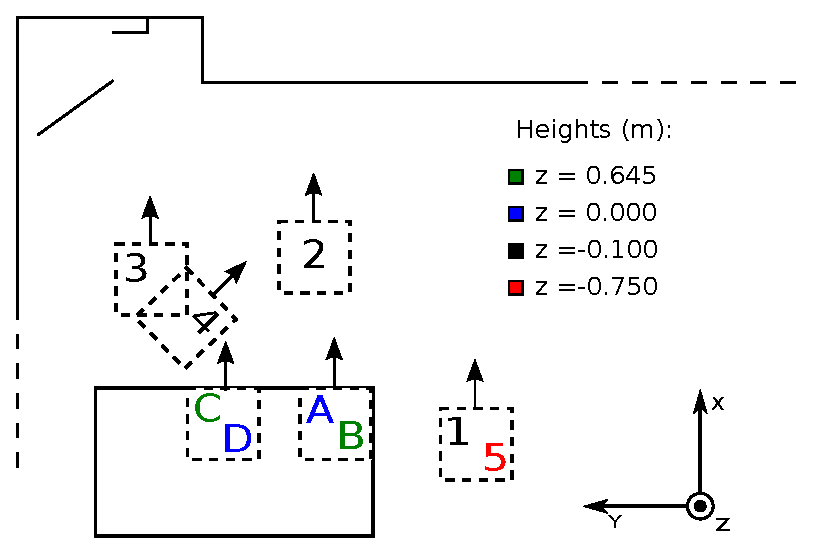
\includegraphics[width=\linewidth]{benchmark_setup.eps}
  \caption{Different positions of the drone during benchmark test}
  \label{fig:benchmarksetup}
\end{subfigure}\\
\vspace{20 mm}
\begin{subfigure}{.33\textwidth}
  \centering
  \includegraphics[width=.99\linewidth]{posA.png}
  \caption{View from position A}
  \label{fig:viewA}
\end{subfigure}%
\begin{subfigure}{.33\textwidth}
  \centering
  \includegraphics[width=.99\linewidth]{posB.png}
  \caption{View from position B}
  \label{fig:viewB}
\end{subfigure}%
\begin{subfigure}{.33\textwidth}
  \centering
  \includegraphics[width=.99\linewidth]{posC.png}
  \caption{View from position C}
  \label{fig:viewC}
\end{subfigure} \\

\begin{subfigure}{.33\textwidth}
  \centering
  \includegraphics[width=.99\linewidth]{posD.png}
  \caption{View from position D}
  \label{fig:viewD}
\end{subfigure}%
\begin{subfigure}{.33\textwidth}
  \centering
  \includegraphics[width=.99\linewidth]{pos1.png}
  \caption{View from position 1}
  \label{fig:view1}
\end{subfigure}%
\begin{subfigure}{.33\textwidth}
  \centering
  \includegraphics[width=.99\linewidth]{pos2.png}
  \caption{View from position 2}
  \label{fig:view2}
\end{subfigure} \\

\begin{subfigure}{.33\textwidth}
  \centering
  \includegraphics[width=.99\linewidth]{pos3.png}
  \caption{View from position 3}
  \label{fig:view3}
\end{subfigure}%
\begin{subfigure}{.33\textwidth}
  \centering
  \includegraphics[width=.99\linewidth]{pos4.png}
  \caption{View from position 4}
  \label{fig:view4}
\end{subfigure}%
\begin{subfigure}{.33\textwidth}
  \centering
  \includegraphics[width=.99\linewidth]{pos5.png}
  \caption{View from position 5}
  \label{fig:view5}
\end{subfigure}

\caption{Views during benchmark test}
\label{fig:benchmarkviews}
\end{figure}

\subsection{Comparison of triangulation methods} \label{sec:comparetriang}
Using the evaluation procedure described in section \ref{evalproc}, we can compare midpoint triangulation and optimal correction. A comparison of their performances can be seen on table \ref{fig:triangcompare}.

\begin{table}[H]
  \centering
  \caption{Comparison between triangulation methods}
  \small\addtolength{\tabcolsep}{-2pt}
  \sisetup{round-mode=places, round-precision = 3}
  \begin{tabular}{ @{} l S[table-format=2.2,round-precision=2] S[table-format=2.1,round-precision=1]
                         S[table-format=2.2,round-precision=2] S[table-format=2.1,round-precision=1] @{}  }
    \toprule
    {}                 & \multicolumn{2}{c}{Accuracy} &  \multicolumn{2}{c}{Robustness} \\
    {}                 & {\footnotesize Distance (\si{\meter})} & {\footnotesize Angle}
                       & {\footnotesize Distance (\si{\meter})} & {\footnotesize Angle} \\
    \midrule
    %Midpoint Method    & \num{0.121729436669}  & \num{0.052339119893} & \num{0.844616151792} & \num{0.27019708855} \\ % radian
    %Optimal Correction & \num{0.0988557438948} & \num{0.0406436455673}& \num{0.775954169079} & \num{0.218538344815}\\ % radian
    Midpoint Method    & \num{0.121729436669}  & \SI{2.9988106732981}{\degree} & \num{0.844616151792} & \SI{15.48115281064}{\degree}\\
    Optimal Correction & \num{0.0988557438948} & \SI{2.3287093550318}{\degree} & \num{0.775954169079} & \SI{12.52132481967}{\degree}\\
      \bottomrule
  \end{tabular}
  \label{fig:triangcompare}
\end{table}

%optimal correc: 24ms
%midpoint      : 12ms

%TODO: put number of matches
We can see that the optimal correction method performs somewhat better. However, this comes at the cost of computation time, because it takes approximately \SI{12}{\milli\second} to triangulate all \num{165} matches between two views using the midpoint method, and \SI{24}{\milli\second} to do the same with the optimal corrction method. In both cases however, this time is insignificant when compared to bundle adjustment (which is performed just after triangulation). For this reason, and the fact that optimal correction is better motivated theoretically and that is gives slightly better results on the benchmark test, we will use optimal correction.\\
It is interesting to see, however, that the difference in performance is much greater between the accuracy and robustness tests than between the two triangulation method. This can be explained by the fact that optimal correction is well suited to correct measurement errors by the camera that follow a normal distribution, but not errors stemming from the fact that the position estimate of the cameras is wrong. That is the reason we need bundle adjustment.

\subsection{Bundle Adjustment}
\begin{table}[H]
  \centering
  \caption{Performance of Bundle Adjustment}
  \small\addtolength{\tabcolsep}{-2pt}
  \sisetup{round-mode=places, round-precision = 3}
  \begin{tabular}{ @{} l S[table-format=2.2,round-precision=2] S[table-format=2.1,round-precision=1] S[table-format=2.3,round-precision=3]
                         S[table-format=2.2,round-precision=2] S[table-format=2.1,round-precision=1] S[table-format=2.3,round-precision=3] @{}  }

    \toprule
    {}      & \multicolumn{3}{c}{Accuracy} &  \multicolumn{3}{c}{Robustness} \\
    {}      & {\scriptsize Distance (\si{\meter})} & {\scriptsize Angle} & {\scriptsize Time (\si{\second})}
            & {\scriptsize Distance (\si{\meter})} & {\scriptsize Angle} & {\scriptsize Time (\si{\second})} \\
    \midrule
    No B.A.  &\num{0.0988557438948}&\SI{2.3287093550318}{\degree}&{\textemdash}&\num{0.775954169079}&\SI{12.52132481967}{\degree}&{\textemdash}\\
    With B.A.&\num{0.0282887755044}&\SI{0.617492395502}{\degree}&\num{0.699653536081}
             &\num{0.0264297442542}&\SI{0.523342243368}{\degree}&\num{2.07235994935}  \\
    \bottomrule
  \end{tabular}
  \label{fig:bacompare}
\end{table}

We see that in the accuracy test, bundle adjustment gives a significant improvement to the performance of the pose estimation. In the robustness test, however, bundle adjustment makes the results quite worse. This is surprising, as it is just in the case where the pose of the camera is uncertain that bundle adjustment should improve the result, by adjusting the pose of the camera. But because the problem is quite non linear, it is possible to fall in local minima. We will later see that by tuning the bundle adjustment phase, we can make it perform much better, and actually improve the results in the robustness test. The other big problem of bundle adjustment is the time it takes. In both tests, this time was over \SI{13}{\second}, which is a prohibitively large amount of time for real time applications. In addition to improving the performance on the robustness test, we will try to reduce the time taken by the bundle adjustment.


\subsection{Tuning the Bundle Adjustment}
The main drawback of Bundle Adjustment is that it requires an iterative method to be solved and can take a lot of time, which of course is a limiting factor for a robot that builds a map in real time. Therefore it is important to optimize both the speed of the computations, and their accuracy. As is often the case, there will have to be a tradeoff between these two goals. To measure both the speed of the Bundle Adjustment and the accuracy of the map obtained, we will conduct some experiments using different parameters to initialize the map.

\subsubsection{Convergence of the solver}
The first element we can tune is the convergence criterion of the solver that solves the bundle adjustment problem. We will stop when the ratio of the change in the objective function to the value of this function arrives below some threshold. This ensures that the criterion scales with the problem, which is important as the size of the problem can vary during operation (as the map grows, for example). The default value of the Ceres solver is $10^{-6}$, but experimentally, we find that we can use a softer threshold to significantly speed up the computations, without impacting the quality of the results too much (and even improving them in the robustness test).

\begin{table}[H]
  \centering
  \caption{Effect of convergence criterion on Bundle Adjustment speed and performance}
  \small\addtolength{\tabcolsep}{-2pt}
  \sisetup{round-mode=places, round-precision = 3}
  \begin{tabular}{ @{} S[scientific-notation=true] S[table-format=1.3] S[table-format=1.3] S[table-format=2.3]
                                                   S[table-format=1.3] S[table-format=1.3] S[table-format=2.3] @{}  }
    \toprule
    \multirow{2}{4em}{Convergence Threshold}  & \multicolumn{3}{c}{Accuracy} &  \multicolumn{3}{c}{Robustness} \\
        & {\scriptsize Distance (\si{\meter})} & {\scriptsize Angle (\si{\radian})} & {\scriptsize Time (\si{\second})}
        & {\scriptsize Distance (\si{\meter})} & {\scriptsize Angle (\si{\radian})} & {\scriptsize Time (\si{\second})} \\
    \midrule
    \num{10}       &\num{0.0988557438948}&\num{0.0406436455673}&\num{0.528740555048}&\num{0.775553503184}&\num{0.219380944042} &\num{0.527468636632} \\
    \num{5}        &\num{0.0988557438948}&\num{0.0406436455673}&\num{0.532568186522}&\num{0.775954169079}&\num{0.218538344815} &\num{0.560289662331} \\
    \num{1}        &\num{0.0988557438948}&\num{0.0406436455673}&\num{0.536680459976}&\num{0.775954169079}&\num{0.218538344815} &\num{0.529257409275} \\
    \num{0.5}      &\num{0.0988557438948}&\num{0.0406436455673}&\num{0.532132491469}&\num{0.284057820455}&\num{0.0860006110714}&\num{0.61461224407}  \\
    \num{0.1}      &\num{0.116334787731} &\num{0.0370860746263}&\num{0.67120449245} &\num{0.244478011775}&\num{0.0982536795903}&\num{1.17620864138}  \\
    \num{0.05}     &\num{0.0684117396072}&\num{0.01622317801}  &\num{0.742543946952}&\num{0.291411483818}&\num{0.112600996782} &\num{2.11719946936}  \\
    \num{0.01}     &\num{0.0895791917611}&\num{0.032296133528} &\num{1.42051474378} &\num{0.823415005012}&\num{0.316300896325} &\num{2.77009601146}  \\
    \num{0.005}    &\num{0.0908954991063}&\num{0.0308365172421}&\num{1.53279625252} &\num{0.142093947791}&\num{0.0495629729962}&\num{4.18590991944}  \\
    \num{0.001}    &\num{0.0849543195902}&\num{0.023134969351} &\num{3.61956872419} &\num{1.034983532}   &\num{0.397193935917} &\num{4.90690393746}  \\
    \num{0.0001}   &\num{0.0842253035954}&\num{0.0258716997751}&\num{5.05812323838} &\num{1.36150222356} &\num{0.479872553731} &\num{10.4840388894}  \\
    \num{0.00001}  &\num{0.0899028376206}&\num{0.0299204957695}&\num{12.4531462789} &\num{1.4834446381}  &\num{0.528430316164} &\num{13.2059885859}  \\
    \num{0.000001} &\num{0.0897626230568}&\num{0.029930165598} &\num{15.7027562261} &\num{1.37414105299} &\num{0.492183127143} &\num{13.8024009466}  \\
    \num{0.0000001}&\num{0.0875171189566}&\num{0.0282118025117}&\num{15.7951563597} &\num{1.55886341652} &\num{0.567309620599} &\num{12.934817493}   \\
    \bottomrule
  \end{tabular}
  \label{tab:convergencetol}
\end{table}

As we can observe on table \ref{tab:convergencetol}, the more severe the convergence threshold, the better the performance on the accuracy test. On the robustness test, however, this is true for high convergence thresholds, but when the convergence threshold is lower than \num{0.01}, the performance starts to degrade as the convergence threshold becomes lower. In both the accuracy and robustness tests, the lower the threshold, the longer it takes. We will chose a threshold of \num{0.05}, as it is a nice compromise of performance on the accuracy test, performance on the robustness test, and speed.


%\chapter{Conclusion} %5
%%%Conclusion (chpt6)
\chapter{Conclusion} %5

In this master's thesis, we achieved our goal of allowing true 3-D SLAM. We are able to build a 3D map based on observations by the monocular camera. To do so, we successfully:
\begin{itemize}
\item Researched the state of the art for monocular visual SLAM
\item Redesigned the keypoint acquisition step to use a more effective hybrid of keypoint tracking and detection
\item Implemented a state-of-the art method for optimal correction when triangulating keypoints
\item Implemented a bundle adjustment step that re-optimizes the map with new information
\item Implemented a mapping strategy that decides when to create keyframe, and when to re-optimize the map with global bundle adjustment
\end{itemize}


The code is now able to build a 3D map using a monocular camera, without making any assumptions regarding the location of keypoints. Using this map, we have shown that the drone can estimate its position very accurately, although at a low frequency. We are able to solve this frequency problem by fusing the visual pose estimation with the IMU, which is available at a much higher frequency, using the pose fusion algorithm created last year.\\

The full mapping algorithm works well for short distances, and we demonstrated that it is conceptually possible for it to work for long trajectories. Unfortunately, due to the unavailable sensors when out of flight, we were not able to show that our full mapping algorithm works during long trajectories. We did show that it could theoretically work during long trajectories by showing that it works when we replace the mapping strategy by a human decision. We are persuaded that if we had access to an ultrasonic sensor, the full mapping algorithm would work, without a human decision maker.\\

We will look at the two main limitations of the current code, and at some possible solutions to these limitations. Then we will look at some ideas to make the current implementation perform better. Finally, we will look at some new directions the UCL's drone project could take in the future years, in particular, what is made possible now that we implemented 3D mapping.\\


\section{Limitations}
The main limitations of our solution, is that with no ultrasound, the mapping algorithm fails on long trajectories, and that the speed of exploration is limited by the time required to run bundle adjustment. We will look at some ways to overcome these limitations.

\subsection{Failure on long trajectories}
In chapter \ref{chpt:results} we were not able to show that our algorithm works during long trajectories. However, we did show that it works on short trajectories, and that if we replace the mapping strategy by a human decision of when to create keyframes (to be able to tell the drone its altitude when keyframes are created), it works quite well. For these reasons, we are convinced that with an available ultrasonic sensor,  the current algorithm would work on long trajectories, and would be able to carry out loop closure.

\subsubsection{Possible solutions}
It would greatly ease development to have access to all sensor data individually, and at any time. This is impossible with the Parrot AR.Drone, because the software running inside is closed-source. Only a change in hardware can really solve this problem, but several solutions are possible:
\begin{itemize}
\item Use another drone, one that has open software, and that is modular so that sensors can be added and removed at will.
\item Attach a new, independent, small ultrasonic sensor to the bottom of the drone, that can communicate its altitude to the drone at all times.
\item Install an external sensor, such as a Kinect\texttrademark , to measure the position of the drone, and use it to simulate the ultrasonic sensor. This would have the added benefit of giving a ground truth of the drone's position at all times, even during displacements.
\end{itemize}

\subsubsection{Computation time of bundle adjustment}
The time taken by bundle adjustment varies widely depending on the number of keyframes considered, the number of points considered, the quality of the initial solution, and the number of bad point matches. In the worst cases, we found that local bundle adjustment could take more than \SI{1}{\second}, which severely impacts the speed at which the drone can explore, because local bundle adjustment is run every time a keyframe is created, and keyframes have to be created frequently enough for all points to be seen from at least two different positions.

\subsubsection{Possible solutions}
Some of the possible ways to reduce the computation time of bundle adjustment are:
\begin{itemize}
\item Further reduce the map to keep only the best points.
\item Reduce the number of keyframes considered during local bundle adjustment. Currently, more keyframes are required to reduce the scale drift (by setting two keyframes constant), but if we had an ultrasound available, it could be used to prevent scale drift, reducing the need for many keyframes during local bundle adjustment.
\item Use a graphics card to parallelize computations.
\end{itemize}

\section{Possible improvements of our implementation}
Here are some ideas that could improve the results of our work, but that weren't tried out:

\subsubsection{Further sanitize the map}
As we could see on the various images of point clouds, many points remain that are behind the wall of the room in which the tests were carried out, which indicates that at least these points don't correspond to real world locations. One idea we did not try out is to remove landmarks that have been present in the map for some time (to be defined) but that were never (or rarely) inliers for RANSAC during localization. This would indicate that they are not useful, and can be removed.

\subsubsection{Changing the type of keypoints}
SIFT keypoints with a SURF detector were chosen last year during one of the master's theses that was written that year. The student who made this choice found that it has the best compromise between performance and complexity. Their have been some important changes to the implementation since then, so it might be interesting to do some experiments with different types of keypoints. For example, ORB keypoints seem to have worked well for other, similar projects.

\subsubsection{A survival-of-the-fittest type strategy for keyframes}
The idea for a survival-of-the-fittest type strategy for keyframes comes from ORB-SLAM \cite{orbslam}. With this strategy, we would create many more keyframes, and then remove all but the "best" ones. This way, we could aim for keyframes placed in space such that there is enough overlap between them, but also such that they are not too close to each other. This would make the need for deciding in advance when to create keyframes less important, moving the decision to later, when there is more information available.

\subsubsection{A separate node for global bundle adjustment}
Because bundle adjustment takes a long time, it is done in a separate node. The mapping node sends part of the map to the bundle adjustment node, which optimizes this part of the map and sends it back to the mapping node. When the mapping node decides to run global bundle adjustment, it simply sends the entire map to the bundle adjustment node. Having a separate node just for global bundle adjustment would allow to run global bundle adjustment in the background permanently. 


\section{Next steps for this project}
There are many different directions that can be taken for the next steps of this project. Here, we highlight some of those that would build on what was achieved in this master's thesis.

\subsubsection{A higher level representation of the map}
Having a real 3D map can be useful for a variety of applications. The current point-cloud configuration of our map well suited for using it to localize the drone by solving the PnP problem, but less suited for other tasks. The point cloud can be transformed to higher level representations, such as a voxel grid. Voxel stands for volumetric pixel, and is a division of 3D space into small units. Such a representation would allow to be able to tell for each point in space whether there is an object there or not, which can then be used for obstacle avoidance. Alternatively, it could be interesting to use the point cloud to determine where walls are, in order to create a human-readable map of a building.\\

\subsubsection{Collaborative mapping}
One of the goals of this project is to enable a group of drones to collaborate. In the previous years, basic communication between drones was implemented, for example allowing them to use a map created by another drone. A more ambitious objective would be for a group of drones to simultaneously build a common map. The implementation of bundle adjustment takes a step in this direction, as we could imagine matching keypoints between keyframes created by two separate drones, resulting in a common map. This would not be trivial, however, as we would need to keep multiple separate maps until there is some overlap between them.

\subsubsection{An Extended Kalman Filter}
The pose estimation coming from PnP alone is not enough to stabilize the drone in flight, as it comes at a frequency too low for the controller. The current pose fusion scheme incorporates the IMU's pose estimation, but does so  with a very basic method. An EKF would significantly improve the accuracy of the fused pose estimation, and allow for a much better controller.

\subsubsection{Hardware change}
A hardware change is always an attractive idea. One of the reasons for a change would be to use a more modular drone, to be able to freely add and remove sensors. Changing the current monocular camera to a stereo or RGB-D camera is tempting, because it lifts the scale uncertainty, and allows to map points from single views, but it should be kept in mind that a monocular camera also has some advantages:
\begin{itemize}
\item They are much more common, making our code useable on a wide variety of devices.
\item The scale ambiguity can also be a monocular camera's strong point: it means that they can be used at any scale, using the same camera, and the same techniques. This is not the case for stereo and RGB-D cameras, which have a maximal and minimal working range.
\item A considerable part of the current code was written specifically for monocular cameras, and would have to be redone in the event of a change.
\end{itemize}

\printbibliography%

%\appendix
%\chapter{Benchmark results}
%\chapter{Full code flowchart}\label{app:flowchart}
\begin{figure}[H]
\centering
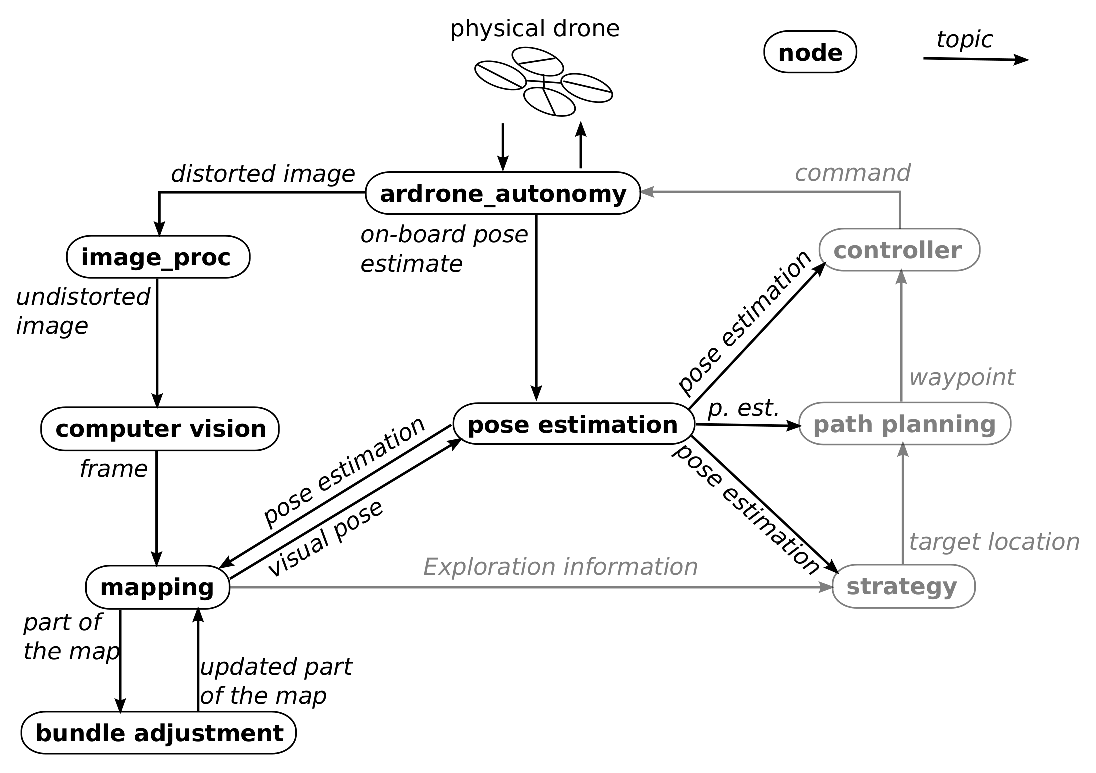
\includegraphics[width=\linewidth]{flowchart.eps}
\caption{Flowchart of the different nodes and the communication between them. Grayed-out parts were not worked on in this master's thesis}
\label{fig:fullflowchart}
\end{figure}


% Back cover page
\backcoverpage

\end{document}
